\section{Echtzeitvisualisierung und OpenGL}
\subsection{Geschichte}
OpenGL entstand ursprünglich aus dem von Silicon Graphics (SGI) entwickelten IRIS GL. Im sogenannten Fahrenheit-Projekt versuchten Microsoft und SGI ihre 3D-Standards zu vereinheitlichen, das Projekt wurde jedoch wegen finanzieller Schwierigkeiten auf Seiten von SGI abgebrochen.

Der OpenGL-Standard wird vom OpenGL ARB (Architecture Review Board) festgelegt. Das ARB existiert seit 1992 und besteht aus einer Reihe von Firmen. Stimmberechtigte Mitglieder sind die Firmen 3DLabs, Apple, AMD/ATI, Dell, IBM, Intel, Nvidia, SGI und Sun (Stand Nov. 2004). Weiter mitwirkende Firmen sind Evans and Sutherland, Imagination Technologies, Matrox, Quantum3D, S3 Graphics, Spinor GmbH, Tungsten Graphics, und Xi Graphics. Microsoft, eines der Gründungsmitglieder, hat das ARB im März 2003 verlassen.

Neue Funktionen in OpenGL werden meist zuerst als herstellerspezifische Erweiterungen eingeführt und gehen dann den Weg über herstellerübergreifende Erweiterungen und ARB-Erweiterungen zu Kernfunktionalität. Dies erlaubt es, neueste Möglichkeiten der Grafikhardware zu nutzen und dennoch OpenGL abstrakt genug zu halten.

Quelle: https://de.wikipedia.org/wiki/OpenGL
\subsection{GL-Pipeline}
Eine Computergrafik-Pipeline besteht im Wesentlichen aus den folgenden Schritten:
\begin{figure}[H]
    \centering
    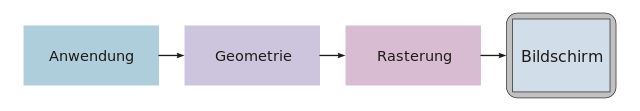
\includegraphics[width=1.0\textwidth]{images/cgpipeline_grob.png}
    \caption{Computergrafik-Pipeline}
    \label{fig:cdpipeline-overview}
\end{figure}

Eine solche Pipeline wird auch von OpenGL implementiert. Es besteht jedoch die Besonderheit, dass die Geometrie und die  Rasterung in Hardware realisiert ist und man durch kleine Programme, sogenannte Shader, auf diese Hardware zugreifen und Manipulationen vornehmen kann beziehungsweise seit OpenGL 2.0 sogar muss.



\subsubsection{Geometrie}
Die Geometrieverarbeitung   besteht aus der Hintereinanderausführung der folgenden affinen/homogenen Abbildungen und Algorithmen:
\begin{figure}[H]
    \centering
    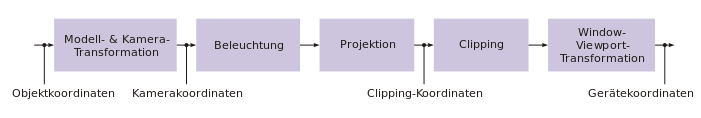
\includegraphics[width=1.0\textwidth]{images/cgpipeline.png}
    \caption{Geometrie-Pipeline}
    \label{fig:cgpipeline-geometry}
\end{figure}

\subsubsection*{Modell und Kameratransformationen}
Die Transformationen von Objektkoordinaten in das Kamerakoordinatensystem werden durch affine Transformationen beschrieben, welche durch Multiplikation durch homogene $4 \times 4$-Matrizen realisiert werden. 

\subsubsection*{Projektion}
Die Projektion wird durch Matrizen ähnlich der Projektionsmatrix 
$K_{persp_{xy}}$ und $K_{orth_{xy}}$ aus Abschnitt 
\ref{subsub:math:affine-space:homog-coords-projection} realisiert. 
Es werden jedoch noch  Translationen, Rotationen Stauchungen 
dazwischengeschaltet, die ebenfalls als $4 \times 4$-Matrizen realisiert werden 
können und mit denen diese Matrix multipliziert werden. 
Man erreicht damit, dass der Kegelstumpf zwischen der vorderen 
(\textit{nearplane}) und der hinteren (\textit{farplane}) Projektionsebene in 
den $[-1,1] \times [-1,1] \times [-1,1] $ Würfel abgebildet wird, welcher auch 
Sichtvolumen genannt wird. 
\begin{figure}[H]
    \centering
    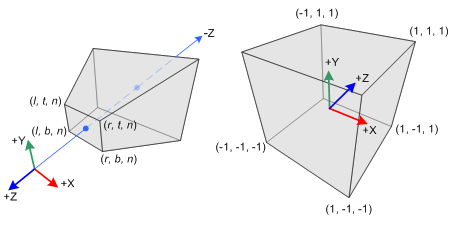
\includegraphics[width=1.0\textwidth]{images/gl_projectionmatrix01.png}
    \caption{Projektion und Sichtvolumen}
    \label{fig:projection-sight-vol}
\end{figure}

Die Multiplikation all diese Matrizen wird auch die MODEL-VIEW-PROJECTION-MATRIX genannt. 

\subsubsection*{Windows-Viewport-Transformation}
Zuletzt müssen die zweidimensionalen Punkte noch mit Hilfe einer 
zweidimensionalen affinen Transformation in das Koordinatensystems des 
Anzeigenfensters auf dem Ausgabegerät transformiert werden. 
Diese Transformation wird auch Windows-Viewport-Transformation genannt.

\subsubsection{Rasterung}
\begin{figure}[H]
    \centering
    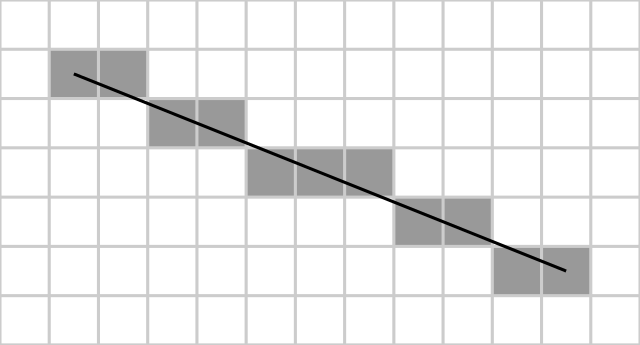
\includegraphics[width=1.0\textwidth]{images/bresenham.png}
    \caption{Rasterung nach Bresenham Algorithmus}
    \label{fig:screening-bresenham-line}
\end{figure}
Als Rasterung bezeichnet man das Transformieren kontinuierlicher, 
zweidimensionaler Daten auf diskrete Pixel. 
Anhand der gegebenen Daten muss also entschieden werden, welche Farbe ein Pixel des Ausgabegerätes erhält.
Wir haben also eine Funktion 
$Frame-Buffer: \mathbb{N} \times \mathbb{N} \to Farbe$. 
Im Bereich Echtzeitvisualisierung sind alle gängigen Rasterverfahren für 
Dreiecke und andere primitiven im wesentlichen Abwandlungen und 
Weiterentwicklungen von Algorithmen, die von Bresenham eingeführt wurden. 
Wir wollen uns den Bresenham Algorithmus für Linien/Strecken dazu exemplarisch 
anschauen.

\begin{Algorithmus}[Bresenham für Strecken mit positiver Steigung]
    \begin{figure}\centering
        \subfloat[Steigungsdreieck]{
            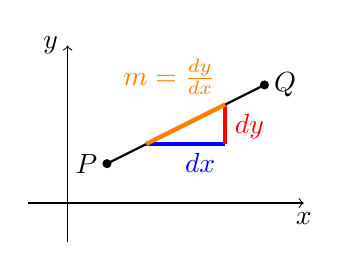
\begin{tikzpicture}[scale=1,]
                % axes
                \draw[->] (-.5, 0) -- (3, 0) coordinate (x axis);
                \node (x-label) at (x axis.south) [anchor=north] {$x$};
                \draw[->] (0, -.5) -- (0, 2) coordinate (y axis);
                \node (y-label) at (y axis.west) [anchor=east] {$y$};
                % S
                \draw[thick, black] (0.5, 0.5) coordinate (P) -- (2.5, 1.5) coordinate (Q);
                \filldraw [black] (P) circle (0.05cm);
                \node (P-label) at (P.west) [anchor=east] {$P$};
                \filldraw [black] (Q) circle (0.05cm);
                \node (Q-label) at (Q.east) [anchor=west] {$Q$};
                % triangle
                \draw[ultra thick, blue] (1, 3/4) -- ++(1, 0) coordinate (dx);
                \node (dx-label) at (dx.south west) [
                    anchor=north east, 
                    color=blue, 
                ] {$dx$};
                \draw[ultra thick, red] (dx) -- ++(0, 1/2) coordinate (dy);
                \node (dy-label) at (dy.south east) [
                    anchor=north west, 
                    color=red, 
                ] {$dy$};
                \draw[ultra thick, orange] (1, 3/4) -- ++(1, 1/2) coordinate (m);
                \node (m-label) at (m.west) [
                    anchor=south east, 
                    color=orange, 
                ] {$m = \frac{dy}{dx}$};
            \end{tikzpicture}
            \label{fig:screening-bresenham-triangle}
        }
        \hspace*{0.1\textwidth}
        \subfloat[Pixelraster]{
            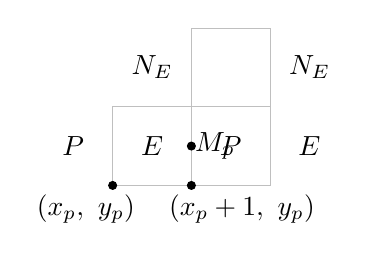
\begin{tikzpicture}
                \foreach \x / \y / \pxname in {-1/-1/P, 0/-1/E, 0/0/N_E} {
                    \draw [lightgray, very thin] (\x, \y) rectangle ++(1, 1);
                    \ifthenelse{\x < 0}{
                        \node (\pxname) at (\x-.5, \y+.5) {$\pxname$};
                    }{
                        \node (\pxname) at (\x+1.5, \y+.5) {$\pxname$};
                    }
                }
                \filldraw [black] (0, -0.5) circle (0.05cm);
                \node (M_p) at (0.3, -0.5) {$M_p$};
                \filldraw [black] (-1, -1) circle (0.05cm);
                \node (x0_y0) at (-1, -1) [
                    anchor=north east, 
                    outer sep=0pt, 
                    xshift=0.4cm, 
                ] {$\left( x_p,~ y_p \right)$};
                \filldraw [black] (0, -1) circle (0.05cm);
                \node (x1_y0) at (0, -1) [
                    anchor=north west, 
                    outer sep=0pt, 
                    xshift=-0.4cm, 
                ] {$\left( x_p + 1,~ y_p \right)$};
            \end{tikzpicture}
            \label{fig:screening-bresenham-pixels}
        }
        \caption{Schrittbetrachtung Bresenham Algorithmus}
        \label{fig:screening-bresenham}
    \end{figure}
    Die Strecke $S = \overline{PQ} \in \mathbb{R}^n$ soll auf ein 
    ($n$-dimensionales Pixel-) Raster abgebildet werden (Siehe Abbildung 
    \ref{fig:screening-bresenham-line}). 
    Wir beschränken uns hier auf die Berechnung im $\mathbb{R}^2$. 
    $P$ und $Q$ seien gegeben mit 
    \begin{equation*}\begin{matrix}
        P = \begin{pmatrix} x_0 \\ y_0 \end{pmatrix} & 
        Q = \begin{pmatrix} x_1 \\ y_1 \end{pmatrix} & 
        \forall x_i, y_i \in \mathbb{R}
    \end{matrix}\end{equation*}
    Die Geradengleichung lässt sich einfach bestimmen (Abbildung 
    \ref{fig:screening-bresenham-triangle}):
    \begin{equation*}\begin{matrix}
        y & = & mx + b \\
        & \textrm{mit} & \\
        m & = & \frac{dy}{dx} \\
        dx & = & x_1 - x_0 \\
        dy & = & y_1 - y_0 \\
    \end{matrix}\end{equation*}
    Die Abbildung auf ein Raster ist für Steigungen 
    $m \in \left\{ 0,~ 1 \right\}$ trivial. 
    Anders für $0 < m < 1$. 
    Dafür betrachten wir in einem Schritt benachbarte Pixel 
    (Abbildung \vref{fig:screening-bresenham-pixels}): 
    \begin{itemize}
        \item Ausgangspixel $P\left( x_p,~ y_p \right)$
        \item Nachbar $E\left( x_p + 1,~ y_p \right)$
        \item ,,Nachfolgender'' Nachbar $N_E\left( x_p + 1,~ y_p + 1 \right)$
    \end{itemize}
    Der Mittelpunkt zwischen $P$ und $E$ wird festgelegt durch
    \begin{equation*}
        M_p = \left( x_p + 1,~ y_p + \frac{1}{2} \right)
    \end{equation*}
    Damit kann entschieden werden welches benachbarte Pixel zur Strecke gehört. 
    Liegt nun
    \begin{equation*}
        M_p ~\Big\{~ \begin{matrix}
            \textrm{oberhalb}~ \overline{PQ} &\Rightarrow& \textrm{wähle}~ E \\ 
            \textrm{unterhalb}~ \overline{PQ} &\Rightarrow& \textrm{wähle}~ N_E 
        \end{matrix}
    \end{equation*}\\
    Bresenham hat eine effiziente Lösung dieses Problems aufgezeigt.
    Zunächst lässt sich die Geradengleichung in eine Funktion $F$ umformen, die von 
    zwei Variablen abhängt: 
    \begin{equation*}\begin{matrix}
        y & = & \frac{dy}{dx} x + b \\
        dx \cdot y & = & dy \cdot x + dx \cdot b \\
        0 & = & dy \cdot x - dx \cdot y + dx \cdot b \\
        F\left(x,~ y\right) & := & dy \cdot x - dx \cdot y + dx \cdot b 
    \end{matrix}\end{equation*}
    Das arithmetische Entscheidungskriterium lautet also 
    \begin{equation*}\begin{matrix}
        (x,~ y) \in y = mx + b & \Leftrightarrow & F\left(x,~ y\right) = 0 \\
        & \textrm{bzw.} & \\
        F\left(x,~ y\right) & \Bigg\{ & \begin{matrix}
            = 0 & \left(x,~ y\right) \textrm{liegt auf}~ S \\
            > 0 & \left(x,~ y\right) \textrm{liegt unterhalb von}~ S \\
            < 0 & \left(x,~ y\right) \textrm{liegt oberhalb von}~ S \\
        \end{matrix}
    \end{matrix}\end{equation*}
    Damit kann die Entscheidungsfunktion $D_p$ definiert werden 
    \begin{equation*}\begin{matrix}
        D_p & := & 2 \cdot F\left(M_p\right) \\
        & = & 2 \cdot F\left(x_p + 1,~ y_p + \frac{1}{2}\right) \\
        & = & dy \left(2x_p + 2\right) - dx \left(2y_p + 1\right) + dx \cdot 2b
    \end{matrix}\end{equation*}
    1. Fall: $D_p < 0 ~\Rightarrow~$ Nachfolgepixel ist $E$
    \begin{equation*}\begin{matrix}
        D_E & = & 2 \cdot F\left(M_E\right) \\
        & = & 2 \cdot F\left(x_p + 2,~ y_p + \frac{1}{2}\right) \\
        & = & dy \cdot \left(2 x_p + 4\right) 
            - dx \cdot \left(2 y_p + 1\right) 
            + 2 \cdot b \cdot dx \\
        & = & D_p + \bigtriangleup_E \\
        & \textrm{mit} & \bigtriangleup_E := 2 \cdot dy
    \end{matrix}\end{equation*}
    2. Fall: $D_p \ge 0 ~\Rightarrow~$ Nachfolgepixel ist $NE$ \\
    \begin{equation*}\begin{matrix}
        D_{NE} & = & 2 \cdot F\left( M_{NE} \right) \\
        & = & D_p + \bigtriangleup_{NE} \\
        & \textrm{mit} & \bigtriangleup_{NE} := 2dy - 2dx
    \end{matrix}\end{equation*}
    Eine Implementierung könnte wie folgt aussehen: 
    \begin{lstlisting}[language=C]
bresenham(x0, y0, x1, y1){
    dx = x1 - x0;
    dy = y1 - y0;
    d = 2*dy - dx; /*F(x0 + 1,y0 + 1/2) | F(x0,y0)=0*/
    deltaE = 2 * dy;
    deltaNE = 2 * (dy - dx);
    x = x0;
    y = y0;
    writepixel(x0, y0);
    while (x < x1) {
        if (d < 0) {
            d += deltaE;
            x++;
        } else {
            d += deltaNE;
            x++; y++;
        }
        writepixel(x, y);
    }
}
    \end{lstlisting}
\end{Algorithmus}

Das Rastern erzeugt oft harte, kantige und ausgefranste Übergange. Diese Effekte bezeichnet man auch als Aliasing. Algorithmen, die diesen Aliasing-Effekten entgegenwirken nennt man auch 
Antialiasing. 
\begin{figure}[H]
    \centering
    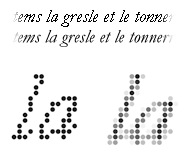
\includegraphics[width=0.5\textwidth]{images/Antialiasing.png}
    \caption{Eine Schrift mit und ohne Antialiasing}
    \label{fig:screening-antialiasing-font}
\end{figure}


\subsection*{Sichtbarkeitsprobleme}

\subsubsection*{Clipping}
Beim 3D-Clipping werden alle Polygone verworfen, die nach der Transformation in Clipping-Koordinaten vollständig ausserhalb des Sichtvolumens
$[-1,1] \times [-1,1] \times [-1,1] $ liegen. Das 2D-Clipping findet nach der Projektion der Polygone statt. Polygone, die über das Viewportfenster hinaus ragen, werden an den Fensterkanten abgeschnitten.
Der wichtigste Schritt ist hierbei das Abschneiden von Strecken an diesen Kanten. Wir betrachten dazu exemplarisch den Cohen-Sutherland-Algorithmus:

\begin{Algorithmus}[Cohen-Sutherland]
\end{Algorithmus}

\subsubsection*{Culling}
Als Culling bezeichnet man das Entfernen von Polygonen anhand Ihrer Orientierung. Man definiert, welche Orientierung eine Rückseite darstellt und verwirft dann Polygone mit dieser Orientierung.

\subsubsection* {z-Buffer}
Der Z-Buffer enthält für jedes Pixel $(u,v)$ nach der Rasterung  einen Wert zwischen $-1$ und $1$. Dieser Wert  ist der Abstand zum nächsten Punkt eines Polygons  in Clipping-Koordinaten von diesem Pixel auf der Projektionsebene.  Wir haben somit eine Funktion
\begin{align*}
Z-Buffer : \mathbb{N} \times \mathbb{N} \to [-1,1]  \; .
\end{align*}

\begin{figure}[H]
    \centering
    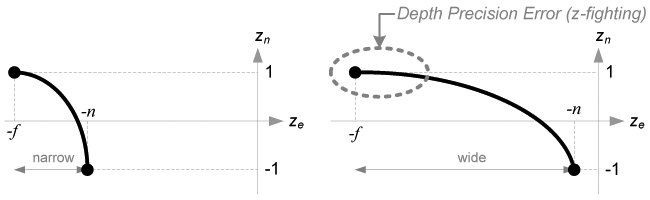
\includegraphics[width=1.0\textwidth]{images/gl_projectionmatrix_zbuffer_1.png}
    \caption{Z-Buffer-War}
    \label{fig:zbuffer-war}
\end{figure}



\begin{Algorithmus}[z-Buffer Algorithmus]
Setze Alle Einträge im Z-Buffer auf 1 (Hintergrund).
Setze alle Einträge im Framebuffer auf die Hintergrundfarbe. \\
$\forall$ Polygone P: \\
begin: \\
Transformiere das Polygon in Clipping-Koordinaten. \\
Transformiere das Polygon in Rasterkoordinaten. \\
$\forall$ erhaltenen Pixel (u,v): \\
begin: \\
$pz := $Z-Koordinate des Polygons in Clipping-Koordinaten zum entsprechenden Pixel \\
$zz:=$ Eintrag im Z-Buffer für das Pixel $(u,v)$ \\
if $pz < zz$: \\
begin: \\
$Z-Buffer(u,v) := pz$ \\
$Frame-Buffer(u,v) := Farbe(P,(u,v))$ \\
end \\
end \\
end
\end{Algorithmus}


\subsection{Lokale Beleuchtungsmodelle}
\subsubsection{Ideale und diffuse Reflexionen}
\subsubsection{Lambert  Modell}
\begin{figure}[H]
    \centering
    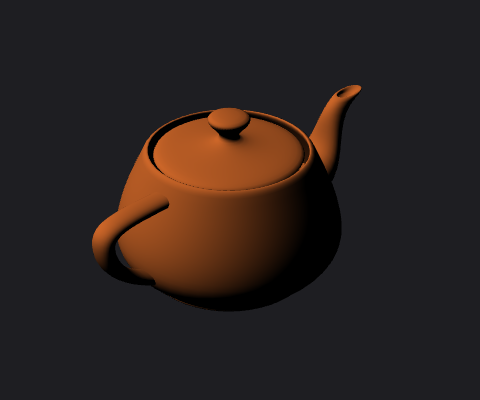
\includegraphics[width=1.0\textwidth]{images/lambert.png}
    \caption{Lambert Modell diffuser Reflektion}
    \label{fig:reflection-lambert-diffuse-model}
\end{figure}


\subsubsection{Phong Modell}
\begin{figure}[H]
    \centering
    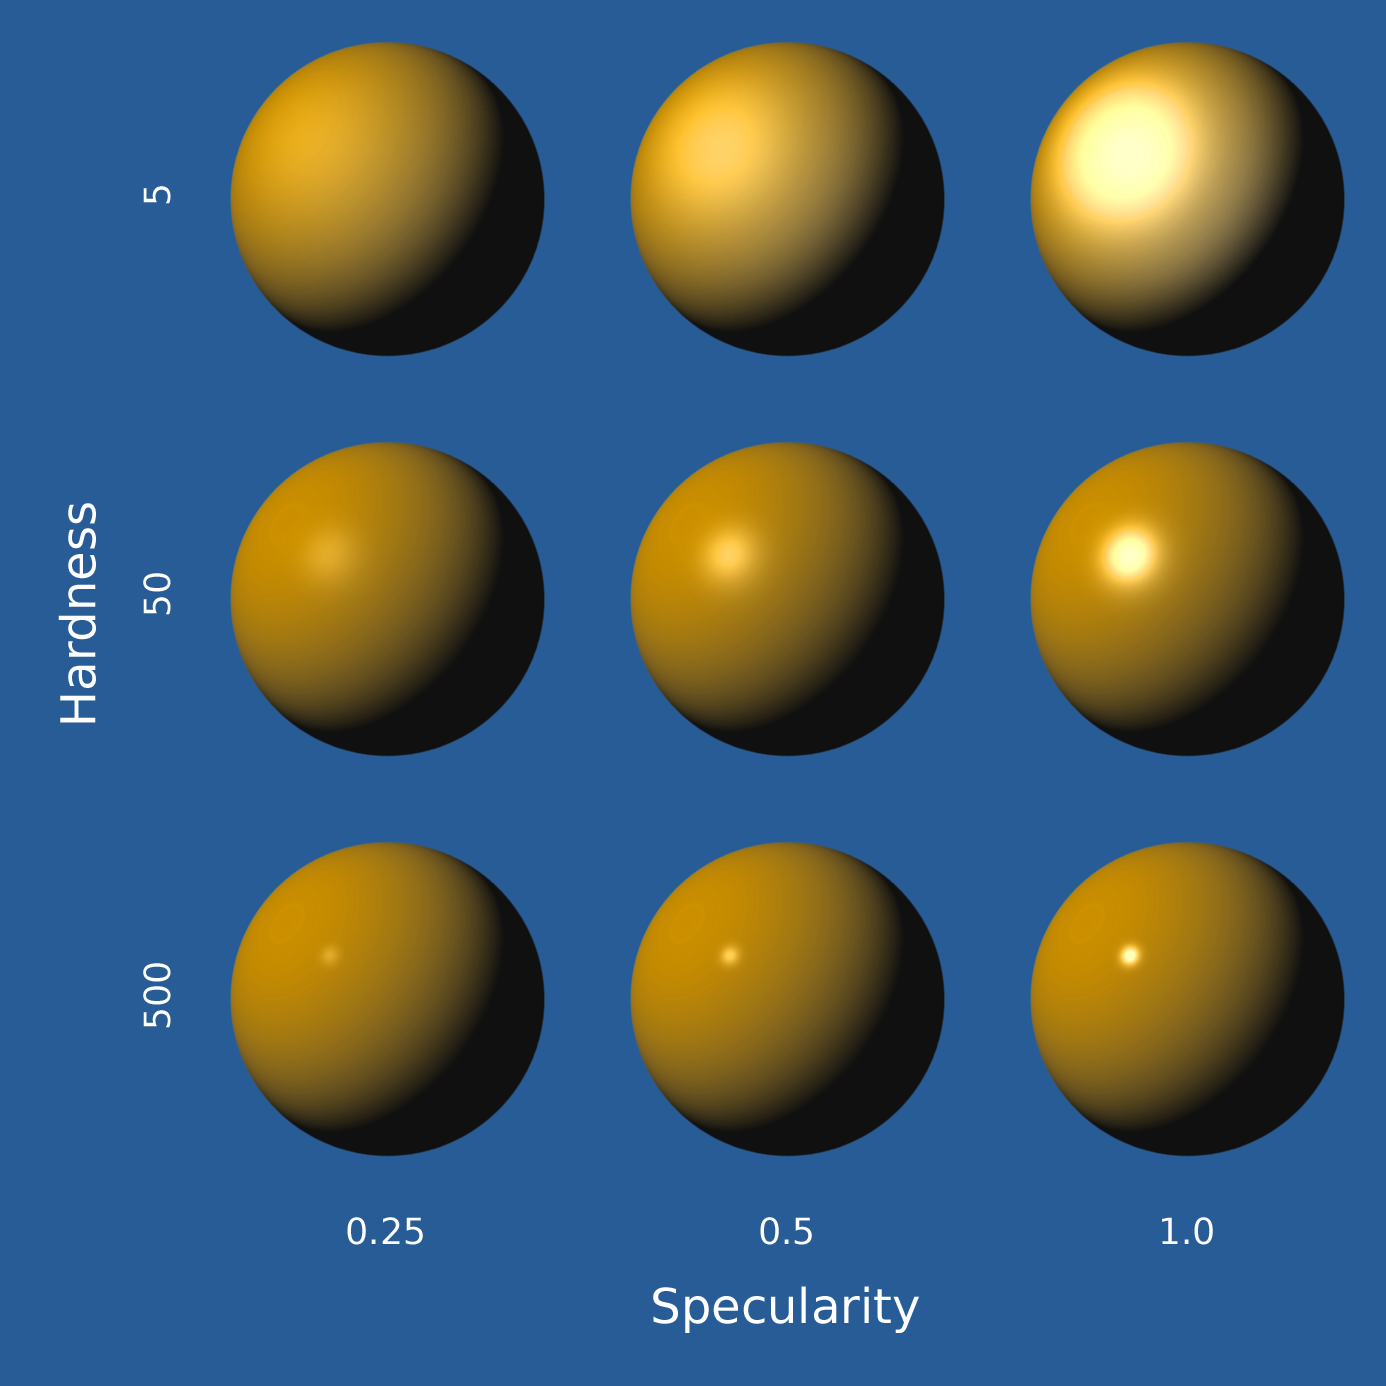
\includegraphics[width=1.0\textwidth]{images/phong.png}
    \caption{Phong Modell spiegelnder Reflektion}
    \label{fig:reflection-phong-specular-model}
\end{figure}





\subsection{Shader und standard Algorithmen}
\subsubsection{Programmierung}

\subsubsection{Shading}
\begin{figure}[H]
    \centering
    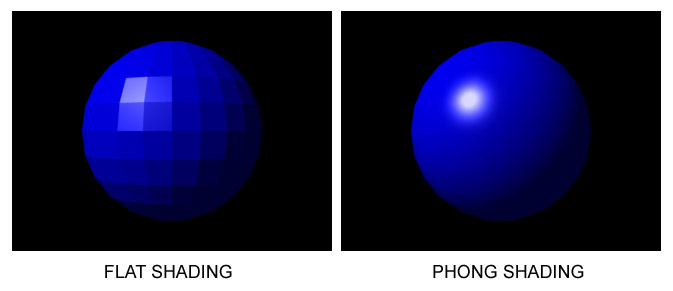
\includegraphics[width=1.0\textwidth]{images/phong_flat_shading.jpg}
    \caption{Flat- und Phong-Shading-Modelle}
    \label{fig:shading-flat-phong-models}
\end{figure}

\subsubsection{Texturen und UV-Mapping}
\begin{figure}[H]
    \centering
    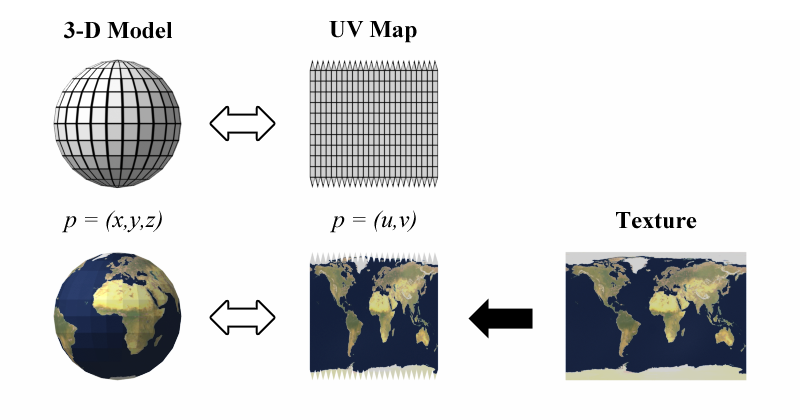
\includegraphics[width=1.0\textwidth]{images/tm_uv.png}
    \caption{uv mapping} %TODO: fix caption&label
    \label{fig:uv-mapping1}
\end{figure}

\begin{figure}[H]
    \centering
    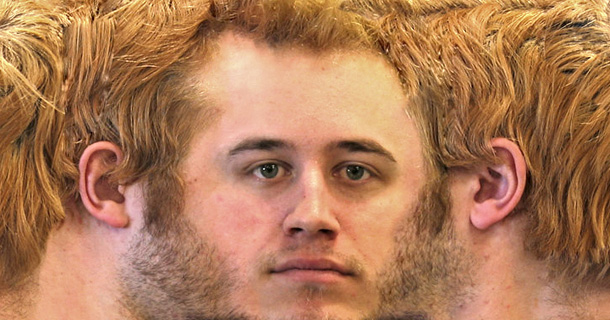
\includegraphics[width=1.0\textwidth]{images/tm_face.jpg}
    \caption{uv mapping} %TODO: fix caption&label
    \label{fig:uv-mapping2}
\end{figure}


\subsubsection{Bumpmapping}
\begin{figure}[H]
    \centering
    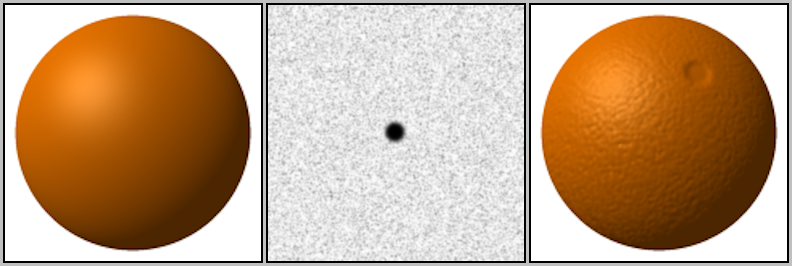
\includegraphics[width=1.0\textwidth]{images/Bumpmap.png}
    \caption{uv mapping} %TODO: fix caption&label
    \label{fig:uv-mapping3}
\end{figure}

\subsubsection{Displacementmapping}



\begin{figure}[H]
    \centering
    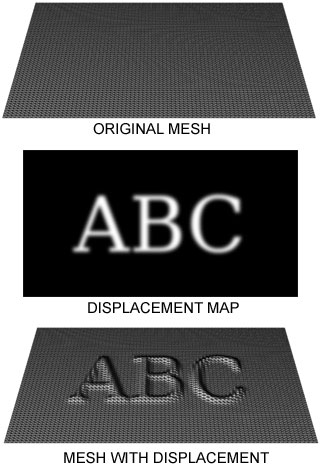
\includegraphics[width=1.0\textwidth]{images/Displacement.jpg}
    \caption{Displacementmapping} %TODO: fix caption&label
    \label{fig:displacement-mapping}
\end{figure}



\subsubsection{Shadowmap}

\subsubsection{Bumpmapping}
\begin{figure}[H]
    \centering
    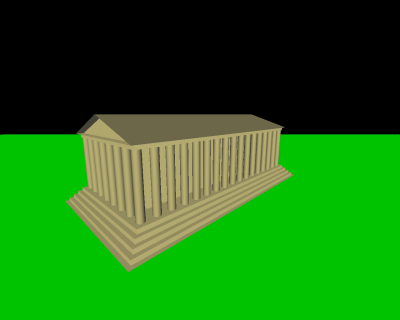
\includegraphics[width=1.0\textwidth]{images/sm_ns.png}
    \caption{shadowmap} %TODO: fix caption&label
    \label{fig:shadowmap1}
\end{figure}

\begin{figure}[H]
    \centering
    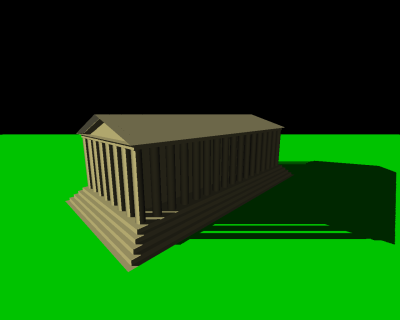
\includegraphics[width=1.0\textwidth]{images/sm_ws.png}
    \caption{shadowmap} %TODO: fix caption&label
    \label{fig:shadowmap2}
\end{figure}

\begin{figure}[H]
    \centering
    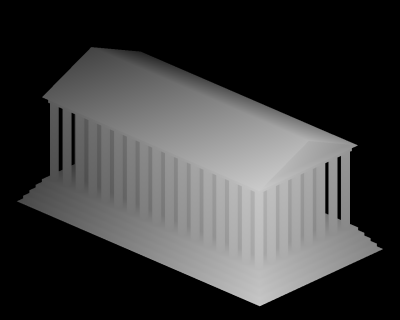
\includegraphics[width=1.0\textwidth]{images/sm_zb.png}
    \caption{shadowmap} %TODO: fix caption&label
    \label{fig:shadowmap3}
\end{figure}


\subsection{GLSL via WebGL}
